%-------------------------------------------------------------------------
\sect{Foundations of the Calculus of Variations}
\label{Foundations of the Calculus of Variations}
%-------------------------------------------------------------------------
\ssect{Preliminaries}
%-------------------------------------------------------------------------

Variational methods can be seen as the fundamental basis for the finite
element method and other numerical techniques. Furthermore, they play
a major role in physics, e.g., it is possible to derive the fundamental 
equations of Newtonian mechanics from a variational principle.

Variational methods can be distinguished between classical methods and
direct methods. 
The classical ones lead to the so-called Euler-Lagrange 
differential equations (Euler differential equations) 
as a necessary condition for the solution of the variational problem. 
Exact solutions
of the differential equations can only be constructed in some simple 
cases. In contrast to this, the direct methods start directly from
the functional. Usually, ansatz-functions with initially unknown
parameters are chosen for the approximation of the real solution.
The parameters can be computed from some necesarry conditions for the 
solution of the variational problem. A popular technique is the
well-known Ritz's method.

In the following we give a brief account of some classical parts
of the calculus of variations. The main task is to find extreme 
values of a functional
\eb
\rm
\Pi(u) = \int_a^b f(x,u(x),u'(x)) \, dx,
\label{functionalpicalcvar}
\ee
where the integrand of $\Pi$ is governed by the unknown function
u(x) and its derivative $\rm u'(x)$. For the function and its derivatives
we have to define some boundary and side conditions. Possible boundary
conditions for u(x) are
\eb
\rm
u(a)=u_a \quad and \quad u(b)=u_b.
\ee

Thus, the main exercise in the calculus of variations is to find a function
u(x) for which the functional $\rm \Pi(u)$ has an extremum, i.e.,
\eb
\rm
\Pi(u) = extreme!.
\label{extrem}
\ee
Functions u(x) satisfying (\ref{extrem}) are the so-called extremals. In the
following we assume that all considered functions are sufficiently
smooth, this means all operations like differentiation and integration
by parts are possible and yield results having the needed properties.

Motivated by the Brachistochrone problem, formulated by Johann Bernoulli (1696),
Euler developed a procedure for the solution of this kind of problems. 
So
his fundamental idea was the construction of a comparable curve $\rm \tilde u(x)$
for the extremal  u(x) with
\eb
\rm
\tilde u(x) = u(x) + \epsilon \eta(x),
\label{vartli}
\ee
where $\epsilon$ is a small value and the arbitrary continuous function
$\eta(x)$ vanishes at the boundaries, see Figure \ref{nfig2_01}.

\begin{Figure}[htb] \unitlength 1 cm
\begin{picture}(12,5.0)
\put( 4.0, 0.0){\scalebox{0.80}{\begin{Figure}[h]
\begin{center}
\unitlength1cm

\begin{picture}(14.0,5.0)
\psfrag{E1}[c][c]{${\bf E}_1$}
\psfrag{E2}[c][c]{${\bf E}_2$}
\psfrag{E3}[c][c]{${\bf E}_3$}
\psfrag{e1}[c][c]{${\bf e}_1$}
\psfrag{e2}[c][c]{${\bf e}_2$}
\psfrag{e3}[c][c]{${\bf e}_3$}
\psfrag{B}[c][c]{${\cal B}$}
\psfrag{S}[c][c]{${\cal S}$}
\psfrag{X}[c][c]{${\bf X}$}
\psfrag{x}[c][c]{${\bf x}$}
\psfrag{M}[c][c]{${\bf M}$}
\psfrag{L}[c][c]{${\BLambda}$}
\psfrag{F}[c][c]{${\bf F}$}
\psfrag{phi}[c][c]{$\Bvarphi_t({\bf X})$}
\put(1.5,0){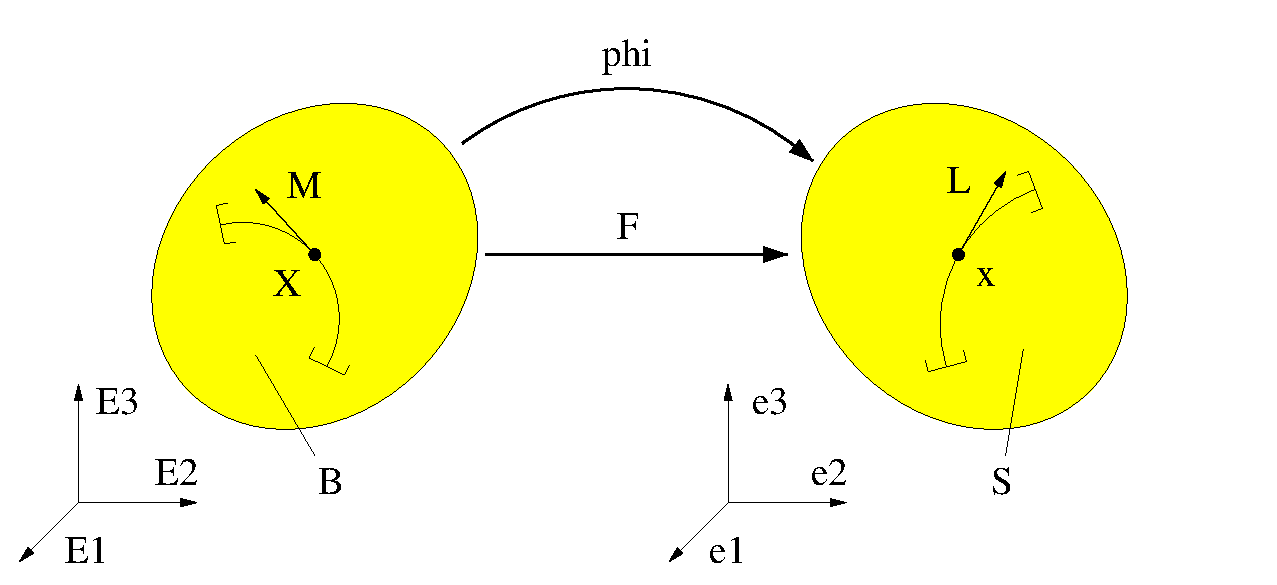
\includegraphics[width=0.75\textwidth]{\dir/config1.eps}}
\end{picture}

\setlength{\baselineskip}{11pt}
\caption{Abbildung der Referenzkonfiguration $\B$ auf die
         Momentankonfiguration ${\cal S}$ mit der nichtlinearen
         Deformationsabbildung $\Bvarphi_t $.
} \label{fig2_01}
\end{center}
\end{Figure}%

%%% Local Variables: 
%%% mode: latex
%%% TeX-master: "sec"
%%% End: 
}}
\end{picture}
\setlength{\baselineskip}{11pt} 
\caption{Boundary conditions $\rm u_a$ and $\rm u_b$, extremal u(x), comparable curve $\rm \tilde u(x)$ and
variation of the extremal $\rm \delta u(x)$}
\label{nfig2_01}
\end{Figure}

For all admissible functions $\rm \tilde u(x)$ the real function 
\eb
\rm
\Pi_{\epsilon}(\epsilon) := 
\Pi(\tilde{u}(x)) =
\Pi(u(x) + \epsilon \eta(x))
\ee
has an extremum for $\epsilon=0$, thus, the necessary condition is 
$
\rm
\left.\! \dfrac{d}{d \epsilon} \Pi_{\epsilon}(\epsilon) \right|_{\epsilon=0} 
\!\! =0.
$ \\
Let us now introduce the notation of the first variation or the so-called 
G\^ateaux-derivative, defined by
\eb
\rm
\displaystyle
\left. \dfrac{d}{d \epsilon} \Pi(u + \epsilon \eta) \right|_{\epsilon=0} 
=
\lim_{\epsilon \rightarrow 0} \dfrac{1}{\epsilon} \left[ \Pi(u + \epsilon \eta) - \Pi(u)\right]
\ee
A necessary condition for the solution of (\ref{extrem}) is that for all admissible comparable functions
$\rm \tilde u(x)$ the G\^ateaux-variation vanishes,
\eb
\rm
\delta \Pi (u;\eta) = 0
\quad\mbox{with}\quad
\delta \Pi (u;\eta)  
=\left. \dfrac{d}{d \epsilon} \Pi(u + \epsilon \eta) \right|_{\epsilon=0} 
\epsilon
, \;
\ee
{\bf Remark:} Formally, k-th order variations of the functional are denoted by
\eb
\rm
\displaystyle
\delta^k \Pi (u;\eta) :=\left. \dfrac{d^k}{d \epsilon^k} \Pi(u + \epsilon \eta) \right|_{\epsilon=0}  \epsilon^k.
\ee

\clearpage
%-------------------------------------------------------------------------
\ssect{Classical Method, Euler-Lagrange Equation}
%-------------------------------------------------------------------------

As pointed above, we seek functions u(x) for which the functional $\rm \Pi(u)$
has an extremum. 
In the following we follow the lines pointed out in standard text books on 
the claculus of variations, e.g.,
Bliss (1962), Weinstock (1974), Bufler (1991), van Brunt (2000),
Lebedev et al. (2003).
For the following analysis we define a comparable function 
(or test function)
\ebn
\rm
\tilde u(x) = u(x) + \epsilon \eta(x),
\een
see (\ref{vartli}) with a small parameter $\epsilon$ and the arbitrary function $\rm \eta(x)$
satisfying the homogenous boundary conditions
\begin{equation}
\rm
\eta(a)=0 \quad \mbox{und} \quad \eta(b)=0 .
\label{bceta}
\end{equation}
As the variation of the extremal we define 
\begin{equation}
\rm
\delta u(x) := \tilde{u}(x) - u(x) = \epsilon \eta(x) ,
\label{eq:deltu}
\end{equation}
where $\rm \delta u(x)$ could be interpreted as a virtual function, satisfying
the homogenous boundary conditions
\begin{equation}
\rm
\delta u(a)=0 \quad \mbox{und} \quad \delta u(b)=0 .
\label{bcetadeltau}
\end{equation}
Inserting the comparable function $\rm \tilde u(x)$ into $\Pi$
leads to the dependency of $\rm \Pi(\tilde u)=\Pi(\epsilon)$. It follows 
\begin{equation}
\rm
\Pi(\tilde{u}) 
= \int_a^b f(x,\tilde{u},\tilde{u}') dx 
= \int_a^b f(x, u+\epsilon \eta, u' + \epsilon \eta') dx 
=: \Pi_{\epsilon}(\epsilon) \, .
\end{equation}
Obviously, we obtain for $\epsilon=0$ the extremum 
$\rm \Pi_{\epsilon}(0)=\Pi(u)$.
A Taylor expansion of $\Pi_{\epsilon}(\epsilon)$ yields
\begin{equation}
\rm
{\Pi_{\epsilon}}(\epsilon)
= {\Pi_{\epsilon}}(0)
+ \left. \frac{d {\Pi_{\epsilon}}}{d \epsilon} \right|_{\epsilon=0}
\epsilon 
+ \frac{1}{2!} \left. \frac{d^2 {\Pi_{\epsilon}}}{d \epsilon^2} 
\right|_{\epsilon=0}  \epsilon^2 
+ \dots ,
\end{equation}
or in a more compact notation
\begin{equation}
\rm
{\Pi_{\epsilon}}(\epsilon) = 
\Pi(u, u') 
+ \delta \Pi(u + \epsilon \eta) 
+ \frac{1}{2!} \delta^2 \Pi(u + \epsilon \eta) 
+ \dots .
\label{eq:piu}
\end{equation}
Interchanging integration and differentiation yields
for the first variation
\begin{eqnarray}
\rm 
\delta \Pi(u) & = &\rm  \epsilon \left. \int_a^b \frac{d}{d \epsilon} f(x, 
\underbrace{\rm u + \epsilon \eta}_{\rm \tilde{u}}, 
\underbrace{\rm u'+ \epsilon \eta'}_{\rm \tilde{u}'}) \right|_{\epsilon=0} dx. \end{eqnarray}
In the latter equation we identify the second argument of f with $\rm \tilde u$ and the third
argument with the derivative of the comparable function
\eb
\rm
\tilde u'(x) = u'(x) + \epsilon \eta'(x),
\ee
so we write, applying the chain rule 
\begin{eqnarray*}
\rm 
\delta \Pi(u) & = & 
\rm  \left. \int_a^b \left( \pp{ \, f}{\tilde{u}}  
\pp{\tilde{u}}{\epsilon} + \pp{ \, f}{\tilde{u}'} \pp{\tilde{u}'}{\epsilon} 
\right)
\right|_{\epsilon=0} dx \,\epsilon
               =  \rm  \left. \int_a^b \left( \pp{ \, f}{\tilde{u}}  
\; \eta + \pp{ \, f}{\tilde{u}'} \; \eta' \right)
\right|_{\epsilon=0} dx \,\epsilon  .
\end{eqnarray*}
Using (\ref{eq:deltu}) and the relation $\rm \delta u'= \epsilon \eta'$
leads to
\begin{equation}
\rm \displaystyle \delta \Pi (u) 
= \int_a^b \left( \pp{ \, f}{u} \; \delta u 
+ \pp{ \, f}{u'} \; \delta u' \right) dx .
\end{equation}
Analogously, the second variation is given by the explicit expression
\eb
\renewcommand{\arraystretch}{2.5}
\begin{array}{ccl}
\rm \displaystyle
\delta^2 \Pi (u) 
& = &\rm 
\left.\displaystyle \int_a^b \left( 
  \frac{\partial^2 \, f }{\partial \tilde u \partial \tilde u}  \eta^2 
+ 2\;\frac{\partial^2 \, f }{\partial \tilde u \partial \tilde u'} \eta \eta' 
+ \frac{\partial^2 \, f }{\partial \tilde u'\partial \tilde u'} \eta'^2\right)
\right|_{\epsilon=0} \, dx \,\epsilon^2 
\\
& = &\rm \displaystyle \int_a^b \left( 
  \frac{\partial^2 \, f }{\partial  u \partial  u}  \delta u^2 
+ 2\;\frac{\partial^2 \, f }{\partial  u \partial  u'} \delta u \delta u' 
+ \frac{\partial^2 \, f }{\partial  u'\partial  u'} \delta u'^2 \right) \, dx .\\
\end{array}
\ee
%%Applying the binominal formula leads to 
%%\begin{eqnarray}
%%\rm
%%\delta^2 \Pi (u) 
%%& = & \rm \int_a^b \left( \delta u \pp{}{u} 
%%+ \delta u' \pp{}{u'} \right)^2 \,f \, dx .
%%\end{eqnarray}
Let us now compute the difference of the functionals
$\rm \Pi(\tilde{u})$ and $\rm\Pi(u) $ using 
(\ref{eq:piu}) with $\rm \Pi_{\epsilon}(\epsilon) = \Pi(\tilde u)$ 
\begin{equation}
\rm
\Pi(\tilde{u}) - \Pi(u) = \delta \Pi (u) + \frac{1}{2!} \delta^2 \Pi(u) + 
\dots .
\end{equation}
The necessary condition for an extreme value of the variational problem  
yields
\begin{equation}
\rm
\delta \Pi (u) = 0  \quad \rightarrow \, 
\int_a^b 
\left( \delta u \pp{ \, f}{u} + \delta u'  \pp{ \, f}{u'} \right) dx = 0 .
\label{eq:dpi0}
\end{equation}

\bigskip
\medskip$\Box$
For the justification of the next steps we consider the 
fundamental lemma of the calculus of variations:
If a continuous function $\rm \phi:[a,b] \rightarrow \IR$ satisfies
\eb
\rm
\int_a^b \phi(x) \; \delta u(x) \; dx =0
\label{fundlemma}
\ee
with a twice-differentiable function $\rm \delta u(x)$ that
vanishes at the boundaries, i.e., $\rm \delta u(a) = \delta u(b) = 0$, then 
$
\rm
\phi(x) \equiv 0
$.
\hfill $\Box$ 

\bigskip
\medskip
An illustration of the quantities occuring in 
(\ref{fundlemma}) is pointed out in Figure (\ref{ten092}).
The proof of this lemma is based on a contrary assumption that
$\rm \phi(x) \ne 0$ while (\ref{fundlemma}) holds, which leads to
a contradiction. In this context we refer to standard text books on calculus
of variations, 
see e.g., 
Lebedev {\it et al.} (2003), van Brunt (2004). 


\begin{Figure}[htb] \unitlength 1 cm
\begin{picture}(12,4.)
\put(5.0, 0.0){\scalebox{1.0}{\input{./sec4_calculus_of_variations/ten092.pstex_t}}}
\end{picture}
\setlength{\baselineskip}{11pt} 
\caption{Visualization of the functions $\rm \phi(x)$ and $\rm \eta(x)$, occuring in the fundamental lemma of the calculus 
of variations}
\label{ten092}
\end{Figure}

In order to derive the Euler-Lagrange differential equation 
we have to reformulate (\ref{eq:dpi0}) in such a way, that 
\eb \rm
\delta \Pi (u) = 0  
\quad \rightarrow \, 
\int_a^b 
\left[ \; \bullet \; \right] \delta u \; dx = 0 
\quad \rightarrow \, 
\left[ \; \bullet \; \right] = 0 .
\ee
is valid.
Thus we firstly
perform a partial integration of the second term in 
$(\ref{eq:dpi0})_2$
\begin{equation}
\rm
\int_a^b \pp{ \, f}{u'} \delta u' dx 
= \int_a^b \pp{ \, f}{u'} d \delta u 
= \left. \pp{ \, f}{u'} \delta u \right|_a^b 
- \int_a^b \delta u \frac{d}{dx} \left( \pp{ \, f}{u'} \right) dx .
\end{equation}
Taking the homogenous boundary conditions (\ref{bcetadeltau}) of 
$\rm \delta u$  into account, i.e.,
\begin{equation}
\rm
\left. \pp{ \, f}{u'} \delta u \right|_a^b = 0 \, , \quad \mbox{because} \;\; 
\delta u(a)=0, \: \delta u(b)=0,
\end{equation}
(\ref{eq:dpi0}) is simplified to 
\begin{equation}
\rm
\delta \Pi(u) 
= \int_a^b \left[ \pp{ \, f}{u} 
- \frac{d}{dx} \left( \pp{ \, f}{u'} \right)  \right] \delta u (x) \; 
dx = 0 \, .
\end{equation}
Applying the fundamental lemma of the calculus of variations 
leads to the Euler-Lagrange differential equation
\begin{equation}
\fbox{$ \rm 
\displaystyle 
\pp{ \, f}{u} - \dfrac{d}{dx} 
\left( \pp{ \, f}{u'} \right) = 0 $} 
\label{eq:fule}
\end{equation}
of the variational problem (\ref{extrem}) with (\ref{functionalpicalcvar}),
where the explixit form of (\ref{eq:fule}) is 
\ebn
\rm
\pp{ \, f}{u} - \dfrac{d}{dx}  \left( \pp{ \, f}{u'} \right)
= 
\pp{ \, f}{u} 
- \dfrac{\partial^2 \, f}{\partial x \partial u'}
- \dfrac{\partial^2 \, f}{\partial u \partial u'} u'
- \dfrac{\partial^2 \, f}{\partial u' \partial u'} u^{\prime \prime} .
\een

\clearpage
As a first application we consider a simple one dimensional truss
of length $\rm l$.
The Young's modulus $\rm E$ is assumed to be constant, the 
cross-sectional area $\rm A(x)$ and the axial loading $\rm p(x)$   
are functions of the location. 

\begin{Figure}[htb] \unitlength 1 cm
\begin{picture}(12,4.)
\put(4.0,0){\scalebox{0.90}{\input{./sec4_calculus_of_variations/ten093.pstex_t}}}
\end{picture}
\setlength{\baselineskip}{11pt} 
\caption{One-dimensional truss with variable stiffness $\rm EA(x)$
and axial loading $\rm p(x)$}
\label{ten093}
\end{Figure}

Furthermore, the displacements of the 
considered system are constrained at both ends of the bar, i.e. 
\begin{equation}
\rm
u(0) = 0 \qquad \mbox{and} \qquad u(l)=0 \, . 
\end{equation}

Let us start from the principle of the minimum of total potential energy 
\begin{equation}
\rm
\Pi(u) = \Pi^i (u) + \Pi^e (u) \rightarrow \mbox{minimum!},
\end{equation}
where 
$ \rm \Pi $
denotes the total potential energy,  
$\rm \Pi^i$
the deformation or strain energy (internal energy)
and $\rm \Pi^e$ the potential of the external loads.
This principle states that a loaded elastic system presents an
equilibrium state under some suitable boundary conditions if the 
total potential energy assumes a stationary value. In the following 
we focus on linear elastic systems; in this case the potential reaches
a minimum.  
The strain energy is given by 
\begin{equation}
\rm
\Pi^i (u) = \dfrac{1}{2}\int_0^l EA(x) u'^2(x) dx 
\end{equation}
and 
the potential of the external loads
has the form
\begin{equation}
\rm
\Pi^e (u) = - \int_0^l p(x) u(x) dx .
\end{equation}
Identifying the integrand of (\ref{functionalpicalcvar})
with the latter equations yields
\eb
\rm
f(x,u,u') = \dfrac{1}{2} EA(x) u'^2 (x) - p(x) u(x). 
\ee
Thus, the derivatives of $\rm f$ with respect to 
$\rm u$ and  $\rm u^{\prime}$ are 
\begin{equation}
\rm
\pp{ \, f}{u} 
= - \, p(x) 
\end{equation}
and 
\begin{equation}
\rm
\frac{d}{dx} \left( \pp{ \, f}{u'} \right) 
= \frac{d}{dx} \left( EA(x) u^{\prime} (x) \right) 
= E (A (x) u' (x) )' \; , 
\end{equation}
respectively. 
Evaluating (\ref{eq:fule}) yields the Euler-Lagrange differential equation 
\begin{equation}
\rm
- \, p(x) - E (A (x) u' (x) )' = 0 
\end{equation}
for the axial displacements of an axially loaded bar. 

% An alternative derivation of this fundamental differential equation is 
% based on the evaluation on the equilibrium conditions. Let us consider
% an infinitesimal bar-element of length $\rm dx$, see Figure \ref{fig2_03}.  
% 
% \begin{Figure}[htb] \unitlength 1 cm
% \begin{picture}(12,2.2)
% \put(5.4,-0.3){\scalebox{1.0}{\input{./sec5/fig2_03.pstex_t}}}
% \end{picture}
% \setlength{\baselineskip}{11pt} 
% \caption{Internal forces at the left-hand and right-hand section.}
% \label{fig2_03}
% \end{Figure}
% 
% 
% The axial internal force acting on the cross-section of the bar is 
% \eb
% \rm
% N(x) = \displaystyle \int_A \sigma (x) dA
% \quad\rightarrow \quad
% N(x) = EA(x) u'(x) ,
% \label{eq:N}
% \ee
% where the axial strain $\rm u'(x)$ is constant over the cross-section.
% In the latter equation we have used Hooke's law
% \eb
% \rm
% \sigma (x) = \displaystyle E u'(x) 
% \ee
% which relates the axial stress $\sigma $ to the axial strain. 
% At the left-hand section we have the internal force $\rm N$ and at the 
% right-hand section $\rm N + d N$. Evaluating the equilibrium condition 
% \eb
% \rm 
% -N + (N + dN) + p \; dx = 0 
% \quad\rightarrow \quad 
% \dfrac{dN(x)}{dx } + p(x) = 0 . 
% \label{equivaribar}
% \end{equation}
% Inserting the definition of internal force 
% (\ref{eq:N}) into the latter equation leads to the  
% Euler-Lagrange differential equation 
% \begin{equation}
% \rm
% \dfrac{d}{dx} [EA(x) u'(x)] + p(x) = 0 \, . 
% \end{equation}

%-------------------------------------------------------------------------
\sssect{Boundary Conditions}
%-------------------------------------------------------------------------

The boundary $\rm \partial \B$ of the (onedimensional) body of 
interest $\rm \B = [a,b]$ is seperated into 
$\rm \partial \B_u$ and $\rm \partial \B_t$, with
\eb\rm 
\partial \B = \partial \B_u \bigcup \partial \B_t
\quad and \quad 
\partial \B_u \bigcap \partial \B_t = \emptyset .
\ee
For the variational problems we have to specify several types of 
boundary conditions. We distinguish between
\begin{center}
\renewcommand{\arraystretch}{1.5}
\begin{tabular}{lp{9.3cm}}
$\rm 1^{st}$ kind bc's: & These are the Dirichlet boundary conditions or the so-called
essential boundary conditions. Here we describe values of the unknown functions u at each
point of the boundary $\rm \partial \B_u$. \\
$\rm 2^{nd}$ kind bc's: & Boundary conditions for the normal derivatives of u applied to the 
points of the boundary $\rm \partial \B_t$ are denoted as the 
Neumann boundary conditions or natural boundary conditions. \\
$\rm 3^{rd}$ kind bc's: & These are mixed boundary conditions, 
Robin/Cauchy-type boundary condition;
they present linear combinations of the $\rm 1^{st}$ and 
$\rm 2^{nd}$ kind bc's.
\end{tabular}
\end{center}
The boundary conditions of the second and third kind are the natural boundary conditions.
Variational problems subjected to the Dirichlet conditions have been discussed in the last
section. Let us now concentrate on a variational problem subjected to Dirichlet 
and Neumann boundary conditions of the form  
\begin{equation}
\rm
\Pi(u) = \int_a^b f(x,u,u') dx + c \cdot u(b) \rightarrow extreme!
\end{equation}
with the constant c and
\eb
\rm
u(a)=u_a \;\; \rightarrow \;\; 
\delta u(a) =0 \quad  and \quad  \delta u(b) \neq 0.
\ee
The necessary condition for an extreme value is $\delta \Pi = 0$. After integration by 
parts we get 
\begin{equation}
\rm
\delta \Pi(u) = \int_a^b \left[ \pp{ \, f}{u} - \frac{d}{dx} 
\left( \pp{ \, f}{u'}\right) \right] \delta u \, dx + \left[ c + \pp{f(b)}{u'}
\right] \delta u(b) .
\end{equation}
Applying the fundamental lemma of the calculus of variations yields for arbitrary
$\rm \delta u(b) \neq 0$ the set of equations
\begin{equation} 
\rm \displaystyle 
\pp{ \, f}{u} - \dfrac{d}{dx} \left( \pp{ \, f}{u'} \right) = 0 
\quad and \quad 
\rm c + \displaystyle \pp{f(b)}{u'} = 0 .
\label{eq:fundlem}
\end{equation}
Equation $(\ref{eq:fundlem})_1$ is the Euler-Lagrange differential equation
and $(\ref{eq:fundlem})_2$ represents the natural boundary condition of the second kind.  

\bigskip
As an
example for a variational problem with Neumann boundary conditions 
we consider a one-dimensional bar 
of length $\rm l$ with constant
Young's modulus $\rm E$, varying 
cross-sectional area $\rm A(x)$ and axial loading $\rm p(x)$.    
The displacement of the system is fixed at the left end and 
an external force $\rm F$ is applied at the right end of the bar,
see Figure \ref{fig2_04}.

\begin{Figure}[htb] \unitlength 1 cm
\begin{picture}(12,3.8)
\put(4.3,-0.4){\scalebox{0.90}{\input{./sec4_calculus_of_variations/fig2_04.pstex_t}}}
\end{picture}
\setlength{\baselineskip}{11pt} 
\caption{Bar with Dirichlet (left) and Neumann (right) boundary condition}
\label{fig2_04}
\end{Figure}

Using again the principle of the minimum of total potential energy 
\begin{equation}
\rm
\Pi(u) = \Pi^i (u) + \Pi^e (u) \rightarrow \mbox{minimum!}
\end{equation}
with the internal part 
\eb
\rm
\Pi^i  (u) = \int_{x=0}^l  \dfrac{1}{2} EA(x) u'^2 (x) \; dx  
\ee
and the external part
\eb
\rm
\Pi^e  (u) = \int_{x=0}^l - p(x) u(x)  dx - F \cdot u(l)  
\ee
with the geometrical boundary condition $\rm u(0)=0$.
Evaluating (\ref{eq:fundlem}) with $\rm c = -F$ yields
\begin{equation} 
\renewcommand{\arraystretch}{2.5}
\begin{array}{l}
\rm
-p(x) - E [A(x) u'(x)]' = 0 \\
\rm
-F + EA(l) u'(l) = 0 .
\end{array}
\label{eq:fundlembeisp}
\end{equation}
Equation $(\ref{eq:fundlembeisp})_1$ represents the  
Euler-Lagrange differential equation of the variational problem.
The Neumann boundary condition is reflected by   
$(\ref{eq:fundlembeisp})_2$;
it states that the internal force at the right end of the bar
$\rm N(l) = EA(l) u'(l)$ has to be identical to the applied 
external force $\rm F$.


\clearpage
%-------------------------------------------------------------------------
\sssect{Constraint Conditions}
%-------------------------------------------------------------------------

A variety of applications in the calculus of variations demands the 
consideration of constraints which reduce the space of possible extremals.
This constraints are differential equations,
algebraic conditions and inequalities.
Let us consider again a first order variational problem 
with Dirichlet boundary conditions, given by 
\begin{equation}
\rm
\Pi(u) = \displaystyle \int_a^b f(x, u(x), u'(x)) dx \rightarrow extreme!,
\label{eq:nvarprob}
\end{equation}
which is completed by a side condition, here e.g. a differential equation
of the form
\eb
\rm
g(x, u(x), u'(x)) = 0.
\label{eq:nvarprob1}
\ee
In this situation we cannot use the classical concept based on the 
comparable curve $\rm \tilde u(x)$, see (\ref{vartli}), because it does 
not fulfill the side condition. A possibility is the introduction of 
a modified comparable curve 
\ebn
\rm
\tilde{\tilde u}(x) = u(x) + \epsilon_1 \eta_1 (x)+ \epsilon_2 \eta_2 (x).
\een
The parameters $\epsilon_1$ and $\epsilon_2$ are dependent 
due to the side condition.

An alternative is based on the Lagrange-Multiplier method. 
The problem (\ref{eq:nvarprob}) in addition with (\ref{eq:nvarprob1}) 
is equivalent to 
\begin{equation}
\rm
\mathcal{L}(u, \lambda) = \int_a^b h(x, u(x), u'(x), \lambda (x)) dx
\rightarrow extreme!  ,
\end{equation}
where we have introduced the abbreviation 
\begin{equation}
\rm
h(x, u(x), u'(x), \lambda) = f(x, u(x), u'(x)) 
                           + \lambda(x) \, g(x, u(x), u'(x)).
\end{equation}
The set of independent variables is (u,$\lambda$) with the unknown
extremal variable u and the Lagrange multiplier $\lambda$. 
In this approach we obtain the 
Euler-Lagrange differential equations
\begin{equation} 
\renewcommand{\arraystretch}{2.5}
\begin{array}{rcl}
\displaystyle 
\rm
\pp{h}{u} - \dfrac{d}{dx} \left( \pp{h}{u'} \right) & = &0 
\\ [1.6ex]
\displaystyle
\rm 
\pp{h}{\lambda} \equiv g & = & 0 .
\end{array}
\end{equation}

As an application of a problem with a differential equation as 
side condition we consider a one-dimensional bar
with homogenous Dirichlet boundary conditions, as depicted in Figure 
\ref{ten093}.
As before we use the principle of the minimum of total potential energy 
\begin{equation} 
\rm
\Pi(u, \varepsilon) = 
\displaystyle \int_0^l \left( \dfrac{1}{2} EA(x) \varepsilon^2(x) - 
p(x) u(x) \right) dx 
\rightarrow \mbox{minimum}! ,
\label{eq:nvarprobbsp1}
\end{equation}
where we have introduced an independent field for the strains. 
Additionally, we take  a side condition into account, which relates
the strains $\varepsilon$ to the derivative of the displacement field 
$u'$, i.e. the side condition is 
\begin{equation} 
\rm
g(x, u', \varepsilon) = u' - \varepsilon = 0.
\label{eq:nvarprobbsp2}
\end{equation}
Equivalent to the variational problem with side condition 
\begin{equation} 
\rm
\Pi(u, \varepsilon)  \rightarrow \mbox{minimal}! 
\qquad \mbox{with} \qquad g(x, u', \varepsilon) = 0
\label{eq:nvarprobbsp}
\end{equation}
is the demand  
\begin{equation}
\rm
\mathcal{L}(u, \varepsilon, \lambda) = \int_0^l 
l(x, u, \varepsilon, u', \lambda)
dx 
\rightarrow \mbox{extreme!}.
\end{equation}
Here the integrand of the new functional has the explicit form 
\eb
\rm
l(x, u, \varepsilon, u', \lambda) = \frac{1}{2} EA \varepsilon^2 - p \; u +
\lambda (u' - \varepsilon) 
%%l(x, u, \varepsilon, u', \lambda) = \frac{1}{2} EA(x)
%%\varepsilon^2(x) - p(x) u(x) + \lambda(x) (u'(x) - \varepsilon(x))   
\ee
with the Lagrange-multiplier $\lambda$.
The associated Euler equations of this variational problem are
\begin{equation} 
\renewcommand{\arraystretch}{2.5}
\begin{array}{rclcrcc}
\rm
\displaystyle \pp{l}{u} - \dfrac{d}{dx} \left( \pp{l}{u'} \right)  & = & 0
&  \quad\rightarrow\qquad & 
\rm - p - \lambda' & = & 0 ,
\\ 
\displaystyle \rm \pp{l}{\varepsilon} & = & 0  
& \quad\rightarrow\qquad &  
\rm EA \varepsilon - \lambda & = & 0 ,
\\ 
\displaystyle \rm \pp{l}{\lambda} & = & 0 
& \quad\rightarrow\qquad &  
\rm  u' - \varepsilon & = & 0 . 
\end{array}
\label{eq:neulerglgn}
\end{equation}
The last equation characterizes the relation between the displacements 
and the strains. 
An interpretation of the 
Lagrange-multiplier $\lambda $ is obtained from
the second Euler equation, it is the internal force in the axial direction
$\rm N$. Furthermore, this equation can be seen as the ``constitutive law''
of a linear elastic one-dimensional bar. 
Using the identification $\rm \lambda = N$
we observe that $\ref{eq:neulerglgn}_1$ represents the equilibrium 
condition of the axially loaded bar. 

% %-------------------------------------------------------------------------
% \sssect{Higher Order Variational Problems}
% %-------------------------------------------------------------------------
% 
% 
% In the above section we have discussed  first order variational problems
% that means that only the first derivative $\rm u^\prime $ 
% of the unknown function $\rm u$
% appears in the integrand $\rm f$ 
% of the functional $\Pi $. A variational problem is said to be of
% higher-order, when higher derivatives $ \rm u^{(n)}$  for $ \rm n > 1$ occur 
% in f, i.e.
% \begin{equation}
% \rm
% \Pi(u) = \int_a^b f(x,u,u',..., u^{(n)} ) dx 
% \rightarrow \mbox{extreme!}   \quad\mbox{for}\quad n > 1
% \end{equation}
% with the boundary values
% \eb
% \begin{array}{lcl}
% \rm  u (a) = u_a     , & \phantom{xxxxxxx}   & \rm  u (b) = u_b  \\ 
% \rm  u^{\prime} (a) = u^{\prime}_a  , & \phantom{xxxxxxx}   
%          & \rm  u^{\prime} (b) = u^{\prime}_b  \\ 
% ...                                , & \phantom{xxxxxxx}   
%          & ...                               \\ 
% \rm  u^{(n-1)} (a) = u^{(n-1)}_a  , & \phantom{xxxxxxx}   
%          & \rm  u^{(n-1)} (b) = u^{(n-1)}_b .   
% \end{array}
% \ee
% From these relation we conclude that the associated comparable 
% functions and their derivatives up to the order of (n-1) vanish at the
% boundaries.
% In the following we focus on  second-order variational problems
% (n = 2).
% The first variation $\delta \Pi (u) = 0$ is, after 
% interchanging integration and differentiation, given by
% \begin{eqnarray*}
% \rm 
% \delta \Pi(u) & = &\rm  \epsilon \left. \int_a^b \frac{d}{d \epsilon} f(x, 
% \underbrace{\rm u + \epsilon \eta}_{\rm \tilde{u}}, 
% \underbrace{\rm u'+ \epsilon \eta'}_{\rm \tilde{u}'},
% \underbrace{\rm u^{\prime\prime}+ \epsilon \eta^{\prime\prime}}_{
% \rm \tilde{u}^{\prime\prime}}
% ) \right|_{\epsilon=0} dx. 
% \end{eqnarray*}
% After some algebraic manipulations we obtain
% \begin{equation}
% \rm \displaystyle \delta \Pi (u) 
% = \int_a^b \left( \pp{ \, f}{u} \; \delta u 
%                 + \pp{ \, f}{u'} \; \delta u' 
%                 + \pp{ \, f}{u^{\prime\prime}} \; \delta u^{\prime\prime}
% \right) dx .
% \end{equation}
% Partial integration of the second term of the latter expression has 
% already been discussed in the previous sections; 
% for the third term we get
% \begin{equation}
% \rm
% \int_a^b \pp{ \, f}{u^{\prime\prime}} \eta^{\prime\prime} dx 
% = \int_a^b \pp{ \, f}{u^{\prime\prime}} d \eta^{\prime} 
% = \left. \pp{ \, f}{u^{\prime\prime}} \eta^{\prime}  \right|_a^b 
% - \int_a^b \eta^{\prime}  \frac{d}{dx} \left( \pp{ \, f}{u^{\prime\prime}} 
% \right) dx .
% \label{secondvariclas}
% \end{equation}
% Taking the homogenous boundary conditions of $\eta^{\prime} $  into account
% yields 
% \begin{equation}
% \rm
% \left. \pp{ \, f}{u^{\prime\prime} } \eta^{\prime}  \right|_a^b = 0 \, , \quad \mbox{because} \;\; 
% \eta^{\prime} (a)=0, \: \eta^{\prime} (b)=0  .
% \end{equation}
% The remaining part in (\ref{secondvariclas}) is modified as follows
% \begin{equation}
% \renewcommand{\arraystretch}{2.9}
% \begin{array}{l}
% \rm\displaystyle
% - \int_a^b 
% \eta^{\prime} \frac{d}{dx} \left( \pp{ \, f}{u^{\prime\prime}} \right) dx 
% =
% - \int_a^b 
% \frac{d}{dx} \left( \pp{ \, f}{u^{\prime\prime}} \right) d \eta 
% = 
% \\ \rm\displaystyle
% \hspace{1.3cm} 
% - \left. \frac{d}{dx}\left( \pp{ \, f}{u^{\prime\prime}} \right)\eta  \right|_a^b 
% + \int_a^b \eta  \frac{d^2}{dx^2} \left( \pp{ \, f}{u^{\prime\prime}} 
% \right) dx 
% = 
% \int_a^b \eta  \frac{d^2}{dx^2} \left( \pp{ \, f}{u^{\prime\prime}} 
% \right) dx ,
% \end{array}
% \label{secondvariclas2term}
% \end{equation}
% due to the homogenuous boundary conditions for the comparable function.
% The final equation is simplified to 
% \begin{equation}
% \rm
% \delta \Pi(u) 
% = \int_a^b \left[ 
%   \pp{ \, f}{u} - \frac{d}{dx} \left( \pp{ \, f}{u'} \right) +
%   \frac{d^2}{dx^2} \left( \pp{ \, f}{u''} \right)
%   \right] \eta (x) dx = 0 \, .
% \end{equation}
% Applying the fundamental lemma of the calculus of variations 
% leads to the Euler-Lagrange differential equation
% \begin{equation}
% \rm
% \pp{ \, f}{u} - \frac{d}{dx} \left( \pp{ \, f}{u'} \right) +
% \frac{d^2}{dx^2} \left( \pp{ \, f}{u''} \right) = 0 .
% \label{elequ} 
% \end{equation}
% 
% As a first example we consider a beam of length l with the deflection w(x), 
% the constant bending rigidity $\rm EI$ and the continuously distributed 
% force $\rm p(x)$.
% 
% \begin{Figure}[htb] \unitlength 1 cm
% \begin{picture}(12,3.3)
% \put(4.5,0){\scalebox{0.80}{\input{./sec5/ten094.pstex_t}}}
% \end{picture}
% \setlength{\baselineskip}{11pt} 
% \caption{Beam with clamped end at the left and simple support at the right}
% \label{ten094}
% \end{Figure}
% 
% \noindent
% The total potential within the framework of the Euler-Bernoulli beam theory is 
% \begin{equation}
% \rm
% \Pi(w) = \int_0^l \frac{1}{2} EI (w'')^2 dx - \int_0^l p \,  w \, dx \; ,
% \end{equation}
% and the geometrical (essential) bounday conditions of the example depicted in Figure \ref{ten094} are
% \eb
% \rm
% w(0) = 0 \, , \quad w'(0 )= 0 \, , \quad w(l )= 0 \, .
% \ee
% Applying the principle of the minimum of the total potential energy requires
% \begin{equation}
% \rm
% \Pi(w) \rightarrow minimal! \quad \rightarrow \quad \delta \Pi = 0.
% \end{equation}
% Let us now derive the associated Euler-Lagrange differential equation. The integral of the second-order
% variational problem is
% \eb
% \rm
% f(w,w'') = \dfrac{1}{2} EI (w'')^2 - p \, w.
% \ee
% Inserting the non-trivial terms
% \eb
% \rm
% \dfrac{\partial \, f}{\partial w} = -p \, ; \;\; \dfrac{d^2}{dx^2} \left( \dfrac{\partial \, f}{\partial w''} \right) = EI w''^{\prime\prime}
% \ee
% in (\ref{elequ}) yields the well-known differential equation
% \eb
% \rm
% EIw'''' - p =0.
% \ee


\newpage
%-------------------------------------------------------------------------
\ssect{Direct Methods}
\label{sec:dirvarmeth}
%-------------------------------------------------------------------------

The direct methods are used for solving the variational problem rather than 
solving the associated Euler-Lagrange differential equations.
Consequently, we start directly from the variational problem, e.g. from
(\ref{functionalpicalcvar}).
In this framework it is possible to specify requirements on the functional,
which are necessary for the existence of solutions, and 
moreover, it is possible to design approximative numerical methods.


%-------------------------------------------------------------------------
\sssect{Ritz's Method}
%-------------------------------------------------------------------------

The basic idea of Ritz's method, also known as  
Rayleigh-Ritz method, is to reduce the variational problem 
of minimizing the functional 
\ebn
\rm
\Pi(u) = \int_a^b f(x,u(x),u'(x)) \, dx,
%\label{functionalpicalcvarritz}
\een
on the space of all feasible functions 
to a problem which deals with the minimizing of the same functional 
on a finite dimensional space.
For this we choose a function 
\begin{equation}
\rm
\bar{u}(x) = N_0(x) + \sum_{i=1}^n c_i N_i(x)
\label{eq:nnaehansatz}
\end{equation}
for an approximate solution of the problem with the yet unknown 
parameters 
$\rm c_i$ for $\rm i=1,...,n$.
Now we have to seek for the parameters which minimize the functional.
For simplicity we firstly focus on pure Dirichlet boundary conditions 
\ebn
\rm
u(a)=u_a \quad and \quad u(b)=u_b.
\een
In order to satisfy the boundary conditions a priori we choose
functions satisfying
\eb
\rm 
N_0(a) = u_a \quad and \quad N_0(b)=u_b ,
\ee
as well as
\eb
\rm 
N_i(a) = N_i(b)= 0  \quad for \quad i = 1, ... n.
\ee
The latter functions, satisfying the homogenous boundary conditions,
the so-called basis functions, are assumed to be linearly independent, i.e.
\eb
\rm
\sum_{i=1}^n c_i N_i(x) = 0 
\quad iff \quad c_i = 0 \quad for \quad i = 1, ...,n .
\ee
Inserting the finite sum into the variational problem 
leads to the approximation
\begin{equation}
\rm
\Pi(u) \approx \Pi(\bar{u}) = \int_a^b f(x, \bar{u}, \bar{u}') dx 
\rightarrow \, \mbox{extreme!}
\end{equation}
The first variation of the approximated problem reads 
\begin{equation}
\rm
\delta\Pi(\bar{u}) = \int_a^b \left( \displaystyle \pp{ \, f}{\bar{u}}
\delta\bar{u} + \displaystyle \pp{ \, f}{\bar{u}'} \delta\bar{u}' 
\right) dx = 0  
\label{eq:nneahprob}
\end{equation}
with the abbreviation
\begin{equation}
\rm
\delta\bar{u}(x) = \sum_{i=1}^n N_i(x) \delta{c}_i .
\end{equation}
Writing out (\ref{eq:nneahprob}) yields with $\rm \Pi(c_1,...,c_n) = \Pi(\bar u)$
\begin{equation}
\rm
\delta \Pi(c_1,...,c_n) =
\sum_{i=1}^n \int_a^b \left( \displaystyle \pp{ \, f}{\bar{u}} N_i 
+ \displaystyle \pp{ \, f}{\bar{u}'} N_i' \right) dx \, \delta{c}_i = 0 .
\label{ritzvareq}
\end{equation}
Alternatively we can write 
\begin{equation}
\rm 
\displaystyle \pp{\Pi(c_1,...,c_n)}{c_i} = \int_a^b \left( \displaystyle
\pp{ \, f}{\bar{u}} N_i + \displaystyle \pp{ \, f}{\bar{u}'} N_i' \right)
dx = 0 \quad \mbox{for} \quad i=1,...,n , 
\label{eq:nkonstc}
\end{equation}
because the values $\rm \delta{c}_i$ for $\rm i=1,...,n$ in (\ref{ritzvareq})
are arbitrary. The latter expression represents a system of n equations with n parameters $\rm c_i$
for $\rm i=1,...,n$. It should be remarked that the system is linear if $\rm f(\bullet)$ is a quadratic form in the unknown 
variables.

For a more detailed look into Ritz's method let us consider an axially loaded bar with constant
axial rigidity EA. At the left end we fix and at the right end we prescribe a displacement, i.e.
\eb
\rm
u(0) = 0 \quad and \quad u(l)=u_b,
\ee
see Figure \ref{fig4_05}.

\begin{Figure}[htb] \unitlength 1 cm
\begin{picture}(12,3.)
\put(4.9,0){\scalebox{0.80}{\input{./sec4_calculus_of_variations/ten101.pstex_t}}}
\end{picture}
\setlength{\baselineskip}{11pt} 
\caption{System and boundary conditions}
\label{fig4_05}
\end{Figure}

The total potential is 
\begin{equation}
\rm
\Pi(u) = \int_0^l \left( \displaystyle \frac{1}{2} EA (u')^2 - p
u \right) dx \rightarrow \, \mbox{minimal!}
\end{equation}
In order to satisfy the essential boundary conditions we choose the linear function
\eb
\rm
N_0(x) = \dfrac{u_b}{l} x.
\ee
Now we will consider a solution in the form of the polynomial 
\begin{equation}
\rm
\bar{u}(x) = N_0(x) + c_1 N_1(x) 
\label{ubaru}
\end{equation}
with the base function 
\eb
\rm
N_1(x)=x(x-l),
\ee
which vanishes at the boundaries. So we get with $\rm \Pi(c_1)=\Pi(\bar u)$ the approximation (\ref{ceins})
\begin{equation}
\rm
\Pi(c_1) = \int_0^l \left( \displaystyle \frac{1}{2} EA 
(\bar{u}'(x))^2 - p \bar{u}(x) \right) dx .
\label{ceins}
\end{equation}
Evaluating (\ref{eq:nkonstc}) yields
\begin{equation} 
\rm
\begin{array}{ll}
\rm \displaystyle \pp{\Pi(c_1)}{c_1} & \rm = \displaystyle \int_0^l \left( 
EA \bar{u}' N_1'
- p N_1 \right) dx  \\ [1.4ex]
 & =\rm  EA \displaystyle \int_0^l \left( ( N_0' + c_1 N_1' ) N_1' - 
 \dfrac{1}{EA} p N_1 \right) dx = 0.
\end{array}
\end{equation}
After some simple manipulations we get
\eb
\rm
c_1 \displaystyle \int_0^l N_1'^2 dx  = \dfrac{p_0}{EA} \int_0^l N_1 dx
- \int_0^l N_0' N_1' dx ,
\ee
which leads to
\eb
\rm
c_1 \left( \displaystyle \frac{1}{3} l^3 \right)  = \displaystyle
\frac{p_0}{EA} \left( \displaystyle - \frac{l^3}{6} \right) - 0 \quad \rightarrow \quad c_1  = - \displaystyle \frac{p_0}{2 EA}.
\ee
Inserting the solution for $\rm c_1$ in (\ref{ubaru}) gives the sought-after solution
\begin{equation}
\rm
\bar{u}(x) = \displaystyle \frac{u_b}{l} x + \displaystyle 
\frac{p}{2 EA} x (l - x).
\end{equation}
In this special case we obtained the exact solution of the variational problem.


% \bigskip
% \noindent
% $\spadesuit$
% {\it {\large Exercices \rm to \ref{sec:dirvarmeth}}}\\
% 
% Consider an axially loaded bar of length $\rm l$  
% fixed at the left end,
% subjected to an external force $\rm F$ at the right end and a constant
% axial loading $\rm p$.    
% Young's modulus $\rm E$ and the cross-sectional area $\rm A$ are constant.
% The total potential energy of the considered boundary value problem 
% is given by 
% \eb
% \rm
% \Pi  (u) = \int_{x=0}^l  \dfrac{1}{2} EA u'^2 (x) \; dx  
%            - \int_{x=0}^l  p(x) u(x)  dx - F \cdot u(l)   .
% \ee
% 
% \begin{Figure}[htb] \unitlength 1 cm
% \begin{picture}(12,4.0)
% \put(4.5,0){\scalebox{0.80}{\input{./sec5/ten103.pstex_t}}}
% \end{picture}
% \setlength{\baselineskip}{11pt} 
% \caption{Axially loaded bar with Dirichlet (left) and Neumann (right) 
% boundary condition}
% \label{ten103}
% \end{Figure}
% 
% Calculate an approximate solution for 
% the axial displacement u(x) using  one
% the parameter function
% \begin{equation}
% \rm
% \bar{u}(x) = c_1 N_1(x)
% \quad \mbox{with} \quad
% N_1 = x 
% \end{equation}
% and the two parameter function
% \begin{equation}
% \rm
% \bar{u}(x) = c_1 N_1(x) + c_2 N_2(x) \quad \mbox{with} \quad
% N_1 = x \, , \, N_2 = x^2 \, .
% \end{equation}
% 




\sssect{Weighted Residual Methods}	

Ritz's method is only applicable if a variational problem exists, which
is equivalent to the considered boundary value problem. For
problems, which cannot be recast into a variational formulation, we
need other methods for the computation of approximate solutions.
Let us consider a differential equation of order  $ 2 k$
\begin{equation}
\rm
f(x, u(x), u'(x),...,u^{(2k)}(x)) + p(x) = 0 \, ,
\label{eq:nmethgewRes}
\end{equation}
in the interval $[a, b]$. The associated 2 k boundary conditions
are alluded to the values of the function u (x)  and/or their
derivatives at the points a and b. For the approximate
solutions we choose an ansatz-function of the form
\begin{equation}
\rm
\bar{u}(x) = N_0(x) + \sum_{i=1}^n c_i N_i(x),
\label{eq:ngewResAnsatz}
\end{equation}
which satisfies all boundary conditions. Furthermore, the
functions $\rm N_0$ and $\rm N_1,..., N_n$ are integrable as well as
their derivations of order $2k$. Inserting the ansatz-function
(\ref{eq:ngewResAnsatz}) in 
(\ref{eq:nmethgewRes}) leads to the so-called residual
\begin{equation}
\rm
r(x) := f(x, \bar{u}(x), \bar{u}'(x),...\bar{u}^{(2k)}(x))
+ p(x) \neq 0.
\label{eq:nRes}
\end{equation}
Now we have to seek the free parameters $\rm c_1, ..., c_n$ in such a
way that the residual is small in some sense. For this we
distribute the residual in an overall manner throughout the
interval. The basic idea is to multiply (\ref{eq:nRes}) with the weighting function $\rm \eta (x)$ and
integrate over the considered domain, i.e.
\begin{equation}
\rm
\int_a^b \eta(x) r(\bar{u}) dx = \int_a^b \eta(x) 
(f(x, \bar{u},...,\bar{u}^{(2k)}) + p(x)) dx = 0 \, .
\label{eq:nGewFunk}
\end{equation}
Based on different definitions of the weighting functions we
obtain different types of approximation methods, e.g. the
point-collocation method, the subdomain-collocation method, the
method of moment, and the Galerkin methods. The weighting function
is chosen by
\begin{equation}
\rm
\eta(x) = \sum_{j=1}^n \bar{c}_j \bar{N}_j(x) \, 
\label{eq:netaAns}
\end{equation}
with the arbitrary parameters $\rm\bar{c} j$. Inserting the weighting
function in the basic equation for the weighted-residual method
(\ref{eq:nGewFunk}) leads to a set of $ n $ equations
\begin{equation}
\renewcommand{\arraystretch}{2.5}
\begin{array}{c}
\displaystyle\rm
\int_a^b \bar{N}_1(x) \; r(x) dx = 0 \\
\displaystyle\rm
\int_a^b \bar{N}_2(x) \; r(x) dx = 0 \\
\displaystyle\rm  
 ...                                       \\
\displaystyle\rm
\int_a^b \bar{N}_n(x) \; r(x) dx = 0 ,\\
\end{array}
\label{eq:nResLoesung}
\end{equation}
which have to be solved with respect to the free parameters 
$ c_1,..., c_n.$

% \medskip
% {\bf Point-Collocation Method}
% 
% The point-collocation method is obtained if we choose the
% Dirac-delta functions
% \eb
% \rm
% \delta (x - x_j)
% \label{eq:LinPC1}
% \ee
% as weighting functions. The defining properties of this function
% are
% \eb
% \rm
% \delta (x - x_j) = 0 \quad {\rm for} \quad x \neq x_j
% \label{eq:LinPC2}
% \ee
% and
% \eb
% \rm
% \displaystyle\int^{\infty}_{- \infty} \delta (x - x_j) d x =
% 1.
% \label{eq:LinPC3}
% \ee
% 
% \begin{figure}[htb] \unitlength 1 cm
% \begin{picture}(12,3.)
% %\put(0,0){X}
% %\put(12,3){X}
% \put(2.,-0.3){\scalebox{0.8}{\input{./sec5/ten107.pstex_t}}}
% \end{picture}
% \setlength{\baselineskip}{11pt} 
% \caption{Weighting function for the point-collocation method}
% \label{ten107}
% \end{figure}
% 
% Using the mean value theorem of the integral calculus and
% performing a limit process yields
% \eb
% \rm
% \displaystyle\int^b_a \delta (x - x_j) r (x) d x = r (x_j).
% \label{eq:LinPC4}
% \ee
% For $\rm x_1, ..., x_n $ collocation points we obtain the set of  n
%  equations
% \begin{equation}
% \renewcommand{\arraystretch}{1.5}
% \begin{array}{c}
% \rm
% r(x_1) := 
% f(x_1, \bar{u}(x_1), \bar{u}'(x_1),...\bar{u}^{(2k)}(x_1)) + p(x_1) = 0    
% \\
% \rm
% r(x_2) := 
% f(x_2, \bar{u}(x_2), \bar{u}'(x_2),...\bar{u}^{(2k)}(x_2)) + p(x_2) = 0    
% \\
% ...
% \\
% \rm
% r(x_n) := 
% f(x_n, \bar{u}(x_n), \bar{u}'(x_n),...\bar{u}^{(2k)}(x_n)) + p(x_n) = 0    
% \\
% \end{array}
% \end{equation}
% with the unknown parameters $\rm  c_1, ..., c_n.$
% 
% If we use step functions instead of the Dirac-delta function we
% obtain the so-called subdomain-collocation method. 
% 
% \begin{figure}[htb] \unitlength 1 cm
% \begin{picture}(12,3.)
% %\put(0,0){X}
% %\put(12,3){X}
% \put(2.,-0.3){\scalebox{0.8}{\input{./sec5/ten105.pstex_t}}}
% \end{picture}
% \setlength{\baselineskip}{11pt} 
% \caption{Weighting function for the subdomain-collocation method}
% \label{ten105}
% \end{figure}
% 
% Applying a set
% of powers of the coordinate variable $\rm x$ for $\rm \eta (x) $ leads to
% the so-called method of moment.
% 
% \bigskip
% {\bf Exemplification:}
% In order to exemplify the point-collocation method we consider a more
% sophisticated problem of an axially loaded bar with Dirichlet boundary 
% conditions and a continuous horizontal elastic foundation 
% (spring parameter k), 
% see Fig. \ref{ten102}.
% 
% \begin{figure}[htb] \unitlength 1 cm
% \begin{picture}(12,4.5)
% \put(2.,0){\scalebox{0.80}{\input{./sec5/ten102.pstex_t}}}
% \end{picture}
% \setlength{\baselineskip}{11pt} 
% \caption{Axially loaded bar with Dirichlet boundary conditions and elastic 
%          support}
% \label{ten102}
% \end{figure}
% 
% 
% The boundary value problem is described by
% \eb
% \rm
% E A \dfrac{d^2 u(x)}{d x^2} - k \, u(x) +  p (x) =0 
% \label{compareexp10}
% \ee
% with the homogeneous essential boundary conditions
% \eb
% \rm
% u(0) = 0 
% \quad\mbox{\rm and}\quad u(l) = 0 \; 
% \ee
% and the linearly varying axial load
% \eb
% \rm
% p (x) = p_0 + \dfrac{\Delta p}{l} x.
% \ee
% For the approximate solution $\rm \bar{u} (x)$, see  
% (\ref{eq:ngewResAnsatz}), we set $\rm N_0 = 0$, and 
% choose an ansatz-function of the form
% \begin{equation}
% \rm
% \bar{u}(x) = \sum_{i=1}^n c_i N_i(x),
% \quad\mbox{with}\quad
% N_i(x) = x^i \; ( l - x ).
% \label{eq:ngewResAnsatzex}
% \end{equation}
% The basis functions are linearly independent and satisfy the homogenous
% boundary conditions $\rm u(0)=0$ and $\rm u(l)=0$.
% For the n collocation points we obtain the residuals
% \eb
% \renewcommand{\arraystretch}{1.5}
% \begin{array}{l}
% \rm
% r( x_1) = EA \bar{u}^{\prime\prime}(x_1) - k~\bar{u}(x_1) + p(x_1) 
% \\
% \rm
% r( x_2) = EA \bar{u}^{\prime\prime}(x_2) - k~\bar{u}(x_2) + p(x_2) 
% \\
% \rm
% ... 
% \\
% \rm
% r( x_n) = EA \bar{u}^{\prime\prime}(x_n) - k~\bar{u}(x_n) + p(x_n),
% \\
% \end{array} 
% \ee
% which are enforced to be zero at the considered points.
% Inserting the ansatz-functions yields the system of equations
% \eb
% \renewcommand{\arraystretch}{1.9}
% \begin{array}{l}
% \displaystyle
% \rm
% EA \sum_{i=1}^{n} c_i~ N^{~\prime\prime}_i(x_1) 
%                          - k~\sum_{i=1}^{n} c_i~ N_i(x_1) = -p(x_1)
% \\
% \displaystyle
% \rm
% EA \sum_{i=1}^{n} c_i~ N^{~\prime\prime}_i(x_2) 
%                          - k~\sum_{i=1}^{n} c_i~ N_i(x_2) = -p(x_2)
% \\
% ...
% \\
% \displaystyle
% \rm
% EA \sum_{i=1}^{n} c_i~ N^{~\prime\prime}_i(x_n) 
%                          - k~\sum_{i=1}^{n} c_i~ N_i(x_n) = -p(x_n)
% \\
% \end{array}
% \ee
% or in the more compact form
% \eb
% \displaystyle
% \rm
% \sum_{i=1}^{n} c_i \bigg( EA ~ N^{~\prime\prime}_i(x_j) 
%                          - k \, N_i(x_j) \bigg) = -p(x_j)
% \quad\mbox{\rm for}\quad j = 1,... ,n.
% \ee
% The unknown coefficients can now be calculated from the system of equations,
% here given in matrix notation, 
% \ebn
% \renewcommand{\arraystretch}{2.0}
% \left[
% \begin{array}{ccc}
% \rm  EA~N^{~\prime\prime}_1 (x_1)-k~N_1(x_1)
% & \cdots
% & \rm EA~N^{~\prime\prime}_n(x_1)-k~N_n(x_1) \\
%   \rm EA~N^{~\prime\prime}_1(x_2)-k~N_1(x_2)
% & \cdots
% & \rm EA~N^{~\prime\prime}_n(x_2)-k~N_n(x_2) \\
% \vdots & \ddots & \vdots \\
%   \rm EA~N^{~\prime\prime}_1(x_n)-k~N_1(x_n)
% & \cdots
% & \rm EA~N^{~\prime\prime}_n(x_n)-k~N_n(x_n) \\
% \end{array}
% \right]
% \left[
% \begin{array}{c}
% \rm c_1\\ \rm c_2\\ \vdots \\ \rm c_n \\
% \end{array}
% \right] =
% \left[
% \begin{array}{c}
% \rm -p(x_1) \\ \rm -p(x_2) \\ \vdots \\ \rm -p(x_n)\\
% \end{array}
% \right]
% \een
% 
% A MATLAB implementation of the method for this special 
% model problem is listed below.
% 
% {\small
% \begin{verbatim}
% % Point-Collocation Method - equidistant collocation points
% % ---------------------------------------------------------
% % parameters: system and loading
% l = 2.0; A = 1.0; E = 1.0; k = 10.0; p0 = 0.1; deltap = 0.1;
% % number of basis functions N_i and collocation points x_j
% n = 6;
% % collocation points, Ansatz functions, first and second derivatives
% for j = 1:n
%   for i = 1:n
%     xcol(i) = i*l/(n + 1);
%     N(j,i)    = xcol(i)^j*(l - xcol(i));
%     Nd(j,i)   = j*xcol(i)^(j - 1)*(l - xcol(i)) - xcol(i)^j;
%     Ndd(j,i)  = j*(j - 1)*xcol(i)^(j - 2)*(l - xcol(i)) ...
%               - 2*j*xcol(i)^(j - 1);
%   end
% end
% % Ndd(1,1) = -2;
% % loading function
% for i = 1:n
%   p(i) = p0 + deltap * xcol(i)/l;
% end
% % system of equations
% for i = 1:n
%   for j = 1:n
%     Amat(i,j) = E*A*Ndd(j,i) - k*N(j,i);
%   end
%   Rvec(i) = -p(i);
% end
% % compute unknowns c_i
% Cvec = Amat\Rvec';
% % continuous Ansatz functions, second derivative and loading function
% x = 0:0.1:l;
% for j = 1:n
%   for i = 1:size(x,2)
%     N(j,i)    = x(i)^j*(l - x(i));
%     Ndd(j,i)  = j*(j - 1)*x(i)^(j - 2)*(l - x(i)) - 2*j*x(i)^(j - 1);
%   end
% end
% for i = 1:size(x,2)
%   p(i) = p0 + deltap * x(i)/l;
% end
% Ndd(1,1) = -2;
% % Approximate solution and residuals
% uapprox  = Cvec'*N;
% residual = E*A*Cvec'*Ndd - k*Cvec'*N + p;
% % Plot
% figure(1)
% plot(x,uapprox)
% xlabel('x')
% ylabel('u(x)','rotation',0)
% figure(2)
% plot(x,residual)
% xlabel('x')
% ylabel('r(x)','rotation',0)
% \end{verbatim}
% }
% 
% 
% equidistant collocation points
% \eb
% \rm
% x_j=\dfrac{j \cdot l}{n+1}
% \ee
% 
% 
% equidistant collocation points with endpoints
% \eb
% \rm
% x_j=\dfrac{(j-1) \cdot l}{n-1}
% \ee
% 
% roots of Tschebyscheff-Polynomials
% \eb
% \rm
% \displaystyle
% x_j=\left( \left( \cos\dfrac{(2j-1)\pi}{2n} \right) +1 \right) \cdot \dfrac{l}{2}
% \ee
% 
% residual norm
% \eb
% e = \sqrt{\int_0^l (r(x))^2~dx}
% \ee
% 
% \begin{figure}[htb] \unitlength 1 cm
% \begin{picture}(12,4.8)
% %\put(0,0){X}
% %\put(12,4.8){X}
% \put(0.0,0){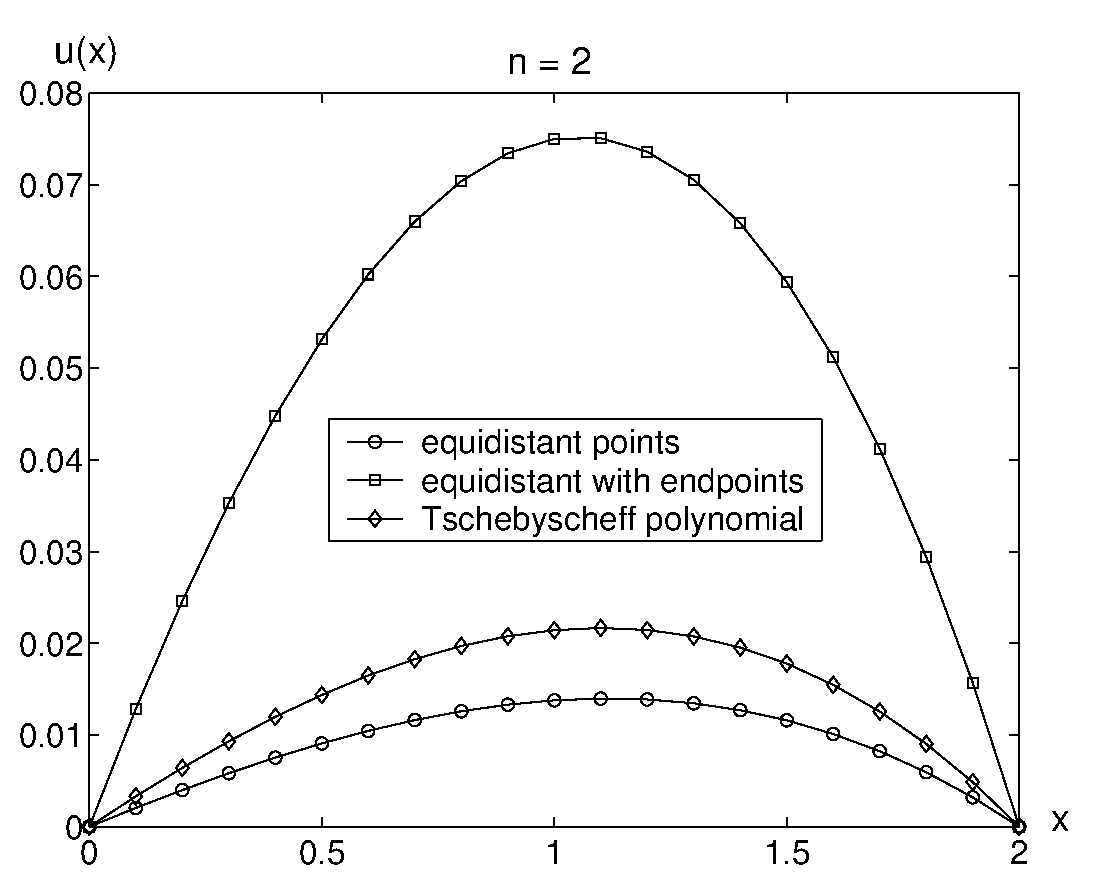
\includegraphics[height=4.6cm]{./sec5/colloc_uapprox_n2.eps}}
% \put(6.0,0){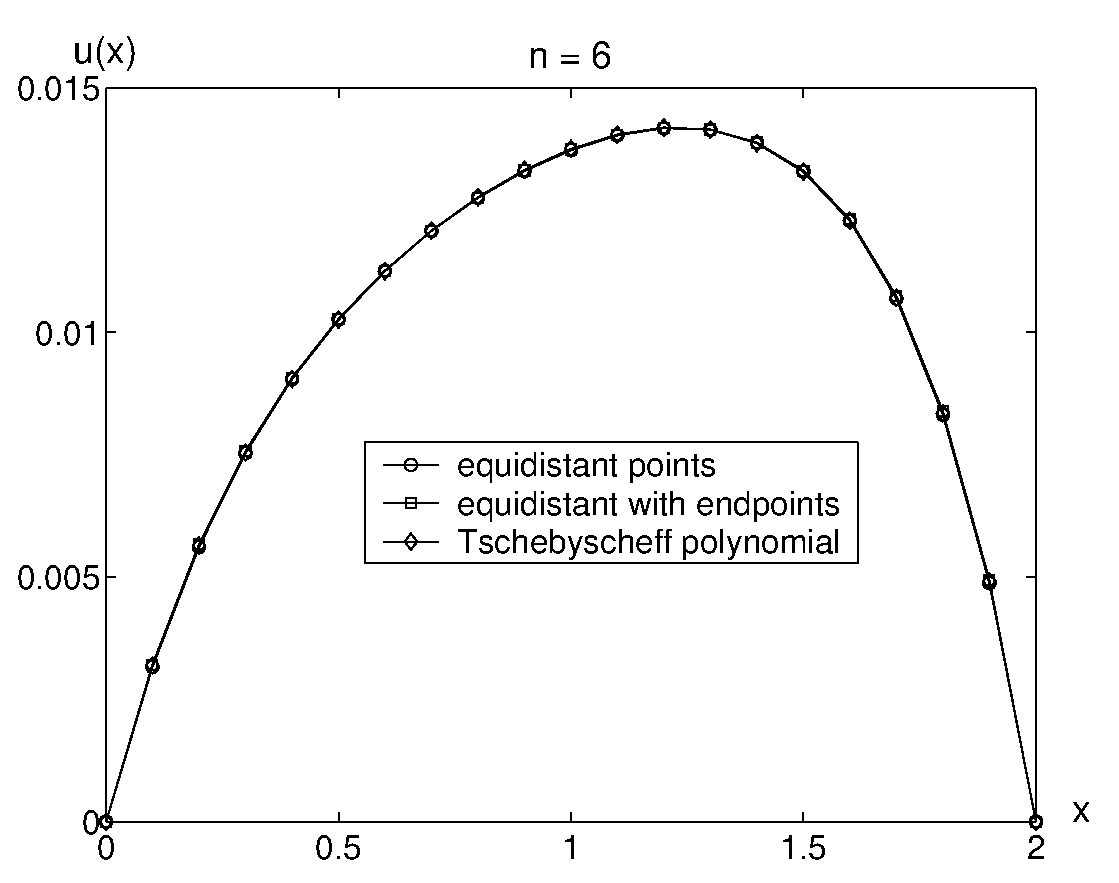
\includegraphics[height=4.6cm]{./sec5/colloc_uapprox_n6.eps}}
% \end{picture}
% \setlength{\baselineskip}{11pt} 
% \caption{Approximate solution for $n=2$ and $n=6$ collocation points}
% %\label{ten}
% \end{figure}
% 
% \begin{figure}[htb] \unitlength 1 cm
% \begin{picture}(12,4.8)
% %\put(0,0){X}
% %\put(12,4.8){X}
% \put(0.0,0){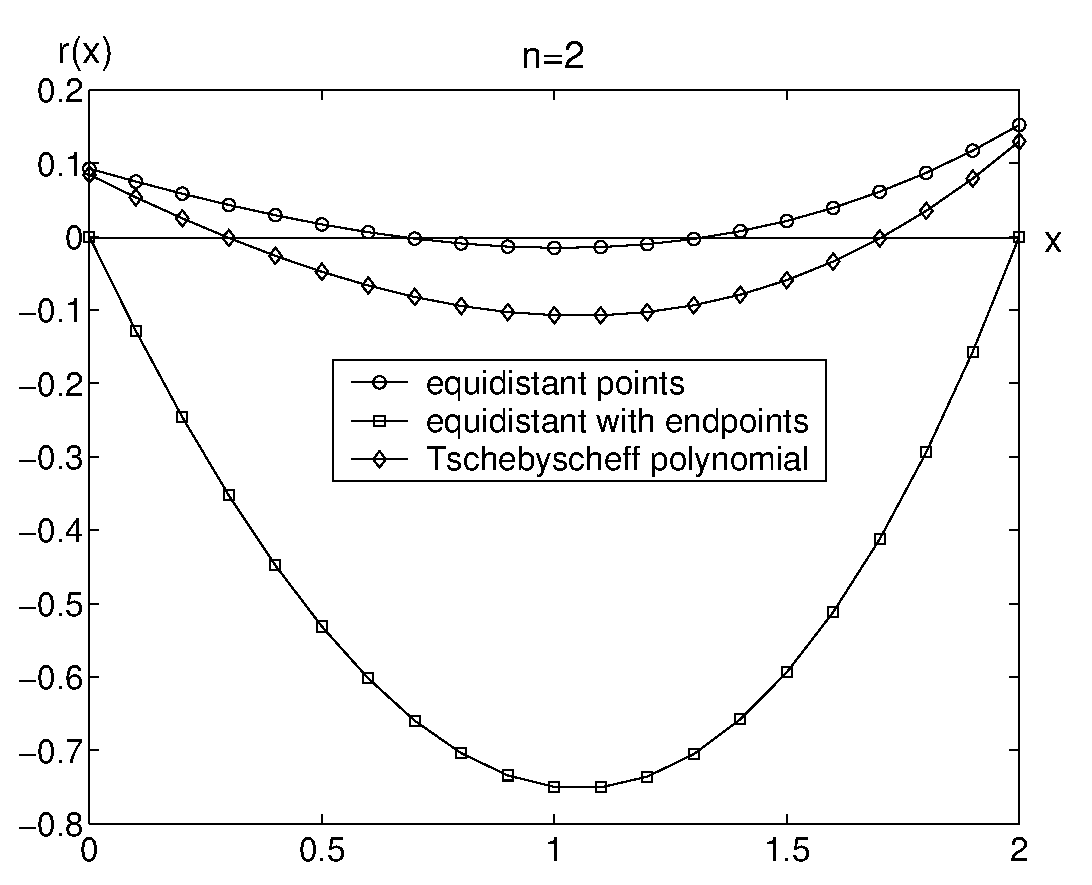
\includegraphics[height=4.6cm]{./sec5/colloc_residual_n2.eps}}
% \put(6.0,0){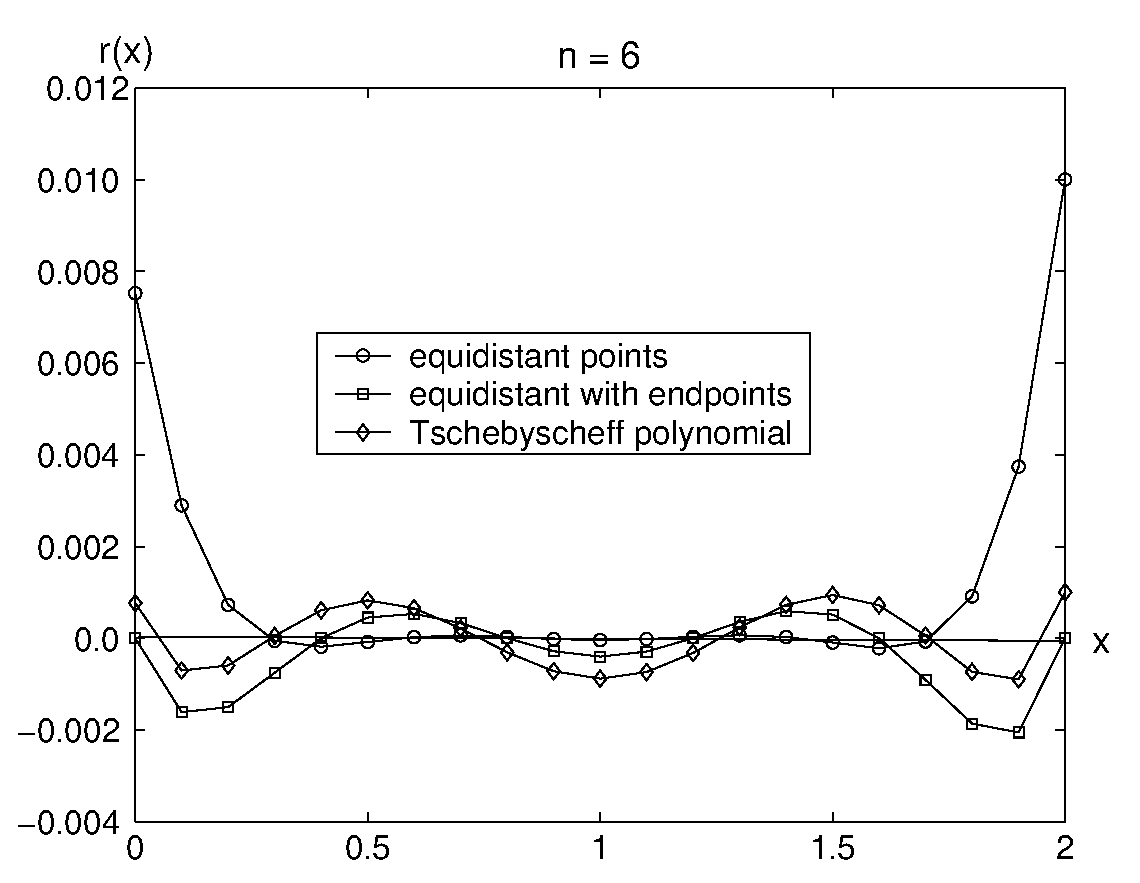
\includegraphics[height=4.6cm]{./sec5/colloc_residual_n6.eps}}
% \end{picture}
% \setlength{\baselineskip}{11pt} 
% \caption{Residuals for $n=2$ and $n=6$ collocation points}
% %\label{ten}
% \end{figure}
% 
% \begin{figure}[htb] \unitlength 1 cm
% \begin{picture}(12,4.8)
% %\put(0,0){X}
% %\put(12,4.8){X}
% \put(3.0,0){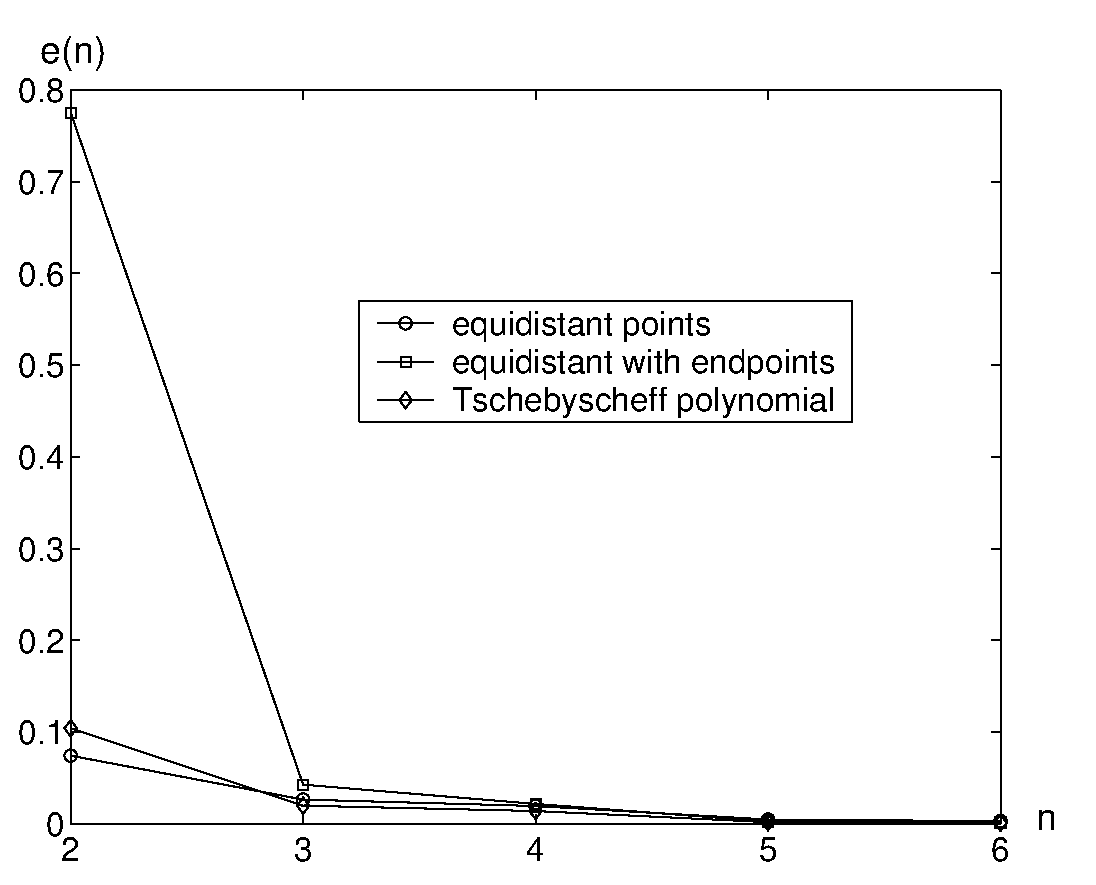
\includegraphics[height=4.6cm]{./sec5/colloc_error.eps}}
% \end{picture}
% \setlength{\baselineskip}{11pt} 
% \caption{Residual norm $e$ for different collocation points}
% %\label{ten}
% \end{figure}
% 

\clearpage
\medskip
{\bf Galerkin Method}

In the Galerkin method the weighting functions are the same as the
approximation basis functions, also known as the Bubnov-Galerkin
method. 

\begin{Figure}[htb] \unitlength 1 cm
\begin{picture}(12,3.)
%\put(0,0){X}
%\put(12,3){X}
\put(4.,-0.3){\scalebox{0.8}{\input{./sec4_calculus_of_variations/ten104.pstex_t}}}
\end{picture}
\setlength{\baselineskip}{11pt} 
\caption{Weighting function for the standard Galerkin method}
\label{ten104}
\end{Figure}

Thus, we obtain with
\eb
\rm
 \bar{N}_i(x) =  N_i(x) \quad\mbox{for}\quad i = 1,2,...,n 
\ee 
the set of equations
\begin{equation}
\renewcommand{\arraystretch}{2.5}
\begin{array}{c}
\displaystyle\rm
\int_a^b {N}_1(x) \; r(x) dx = 0 \\
\displaystyle\rm
\int_a^b {N}_2(x) \; r(x) dx = 0 \\
\displaystyle\rm  
 ...                                       \\
\displaystyle\rm
\int_a^b {N}_n(x) \; r(x) dx = 0 \\
\end{array}
\label{eq:nResLoesunggal}
\end{equation}
An advantage of this method is that an equivalent
variational formulation of the considered boundary value problem
is not required. On the other hand, the ansatz-function have to
fulfill the essential as well as the natural boundary conditions.
Furthermore, for a differential equation of order  2 k, the
functions have to be (2 k - 1)  times continuously
differentiable. This drawback, especially in view of the
Finite-Element-Method, can be avoided by applying partial
integration of the residual function, in general. After this we
can use approximation functions, which have only to be (k - 1) 
times continuously differentiable and only have to satisfy the
essential boundary conditions. 

The latter notes are explained in more detail considering 
the uniform beam fixed at the left end and subjected to 
a vertical point load as well as a bending moment at the other end, 
see Figure \ref{fig4_06}.

\begin{Figure}[htb] \unitlength 1 cm
\begin{picture}(12,3.)
\put(4.5,0){\scalebox{0.80}{\input{./sec4_calculus_of_variations/fig4_06.pstex_t}}}
\end{picture}
\setlength{\baselineskip}{11pt} 
\caption{System and boundary conditions}
\label{fig4_06}
\end{Figure}

The problem is described in terms of the following boundary 
value problem:
\begin{equation} 
\renewcommand{\arraystretch}{1.5}
\begin{array}{rclcl}
\rm EI w''''(x) - p(x) & = &\rm  0       &   & \\ 
\rm              w(0)  & = &\rm  0       &   & \\ 
\rm             w'(0)  & = &\rm  0       &   & \\ 
\rm         EI w''(l)  & = &\rm  -M(l) & ; &\rm   M(l) = M_l \\ 
\rm       EI w'''(l)   & = &\rm  -Q(l) & ; &\rm   Q(l) = F_l \\
\end{array}
\label{eq:nbspprob}
\end{equation}
The essential boundary conditions are $(\ref{eq:nbspprob})_{2,3}$ and the
natural ones are given by $(\ref{eq:nbspprob})_{4,5}$.
Let us now introduce an ansatz-function 
$\tilde{w}$, then the residual of $(\ref{eq:nbspprob})_{1}$ is defined by
\begin{equation}
\rm
r(x) := EI \tilde{w}''''(x) - p(x) .
\end{equation}
Furthermore, the residuals of the equations $(\ref{eq:nbspprob})_{4,5}$ are
\begin{equation}
\rm 
r_M := EI \tilde{w}''(l) + M_l 
\quad \mbox{and} \quad 
r_F := EI \tilde{w}'''(l) + F_l.
\end{equation}
Using the concept of the weighted residual method leads to 
\begin{equation}
\rm
\int_0^l r(x) \eta(x) dx + r_M \eta_M + r_F \eta_F = 0 
\end{equation}
with the weighting function $\rm \eta(x)$ 
and the weights
$\rm \eta_M$ as well as $\rm \eta_F$.
Furthermore, we assume that $\rm \eta(x)$  fulfills the homogeneous boundary 
conditions $\rm\eta(0)=0$ and  $\rm \eta'(0)=0$. 
For the explicit form of this equation we get 
\begin{equation}
\rm  
\int_0^l [EI \tilde{w}''''(x) - p(x)] \eta(x) dx 
+ [EI \tilde{w}''(l) + 
M_l] \eta_M + [EI \tilde{w}'''(l) + F_l] \eta_F = 0
\label{eq:nzwErg1}
\end{equation}
The partial integration of the term  
$\rm\displaystyle\int_0^l EI \tilde{w}''''(x)  \eta(x) dx $ yields
\begin{equation} 
\left. 
\renewcommand{\arraystretch}{1.5}
\begin{array}{ll}
\rm \displaystyle \int_0^l EI \tilde{w}''''(x) \eta(x) dx & = 
\rm \Bigl. EI \tilde{w}'''(x) \eta(x) \Bigr|_0^l - 
\displaystyle \int_0^l EI \tilde{w}'''(x) \eta'(x) dx 
\\ 
              & = 
\rm \Bigl. EI \tilde{w}'''(x) \eta(x) \Bigr|_0^l 
\\ 
              & - 
\rm \Bigl. EI \tilde{w}''(x) \eta'(x) \Bigr|_0^l + 
\displaystyle \int_0^l EI \tilde{w}''(x) \eta''(x) dx
\end{array}
\right\} \, .
\label{eq:nzwErg2}
\end{equation}
After evaluating the boundary terms we get
\begin{equation}
\rm
\int_0^l EI \tilde{w}''''(x) \eta(x) dx = EI \tilde{w}'''(l) \eta(l)
- EI \tilde{w}''(l) \eta'(l) + \int_0^l EI \tilde{w}''(x) \eta''(x) dx  
.
\label{eq:zwErg3}
\end{equation}
Inserting this intermediate result in (\ref{eq:nzwErg1})
\begin{equation} 
\renewcommand{\arraystretch}{1.5}
\begin{array}{l}
\rm \displaystyle \int_0^l [EI \tilde{w}''(x) \eta''(x) - p(x) \eta(x)] dx 
\\ [1.4ex]
\displaystyle
\rm + EI 
\tilde{w}'''(l) [\eta(l) + \eta_F] + \eta_F F_l + EI \tilde{w}''(l) 
[ \eta_M - \eta'(l)] + \eta_M M_l = 0.
\end{array}
\label{eq:nzwErg4}
\end{equation}
For the arbitrary weights
$\rm \eta_M$ and $\rm \eta_F$ we choose 
\begin{equation}
\rm 
\eta_M = \eta'(l) \quad \mbox{and} \quad \eta_F = -\eta(l),
\end{equation}
in order to reduce (\ref{eq:nzwErg4}) to the final expression
\begin{equation}
\rm
\int_0^l [EI \tilde{w}''(x) \eta''(x) - p(x) \eta(x)] dx - \eta(l) F
+\eta'(l) M_l = 0 \, .
\label{eq:nzwErg5}
\end{equation}
It can be seen that the function 
$\rm\tilde{w}(x)$ only has to satisfy the essential boundary conditions
and $\rm \tilde{w}(x)$ and $\rm \eta(x)$ only have to be  
$\rm (k-1)$ times continuously differentiable.


If we choose different functions for the weighting and the
approximation basis functions, i.e.
\eb
\rm
 \bar{N}_i(x) \ne  N_i(x) \quad\mbox{for}\quad i = 1,2,...,n 
\ee 
then the method is dedicated to Petrov-Galerkin.



\bigskip
{\bf Exemplification:}
In order to explain the standard Galerkin method we consider the 
model problem shown in Fig. \ref{ten102}.

\begin{figure}[htb] \unitlength 1 cm
\begin{picture}(12,4.5)
\put(2.,0){\scalebox{0.80}{\input{./sec4_calculus_of_variations/ten102.pstex_t}}}
\end{picture}
\setlength{\baselineskip}{11pt} 
\caption{Axially loaded bar with Dirichlet boundary conditions and elastic 
         support}
\label{ten102}
\end{figure}

Starting from (\ref{eq:nGewFunk}) we obtain for our situation
\begin{equation}
\rm
\int_a^b \eta(x) r(x) dx = 
\int_a^b \eta(x) 
\bigg(
EA \bar{u}^{\prime\prime}(x) - k~\bar{u}(x) + p(x) 
\bigg) 
 dx = 0 \, .
\label{eq:nGewFunkex}
\end{equation}
We can directly use the latter equation for the computation 
of the approximative solution, but in view of the standard procedure 
in the finite-element procedure let us first partially integrate  
$\displaystyle\rm
\int_0^l \eta(x) EA \bar{u}^{\prime\prime}(x) dx 
$:
\eb
 \rm
\int_0^l \eta(x) EA \bar{u}^{\prime\prime}(x) dx 
=
\Bigl.\eta(x) EA \bar{u}^{\prime}(x) \Bigr|_0^l  
-
\int_0^l \eta'(x) EA \bar{u}^{\prime}(x) dx 
\ee
Exploiting the homogeneous conditions 
$\rm \eta(0) = 0$ and $\rm \eta(l) = 0$ yields
\eb
 \rm
\int_0^l \eta(x) EA \bar{u}^{\prime\prime}(x) dx 
=
- \int_0^l \eta^{\prime}(x) EA \bar{u}^{\prime}(x) dx  .
\ee
Thus, the remaining equation reads  
\begin{equation}
\rm
\int_0^l \eta^{\prime}(x) EA \bar{u}^{\prime}(x) dx 
+
\int_0^l \eta(x) ~ k ~\bar{u}(x) dx 
=
\int_0^l \eta(x) p(x) dx.
\label{eq:nGewFunkexex}
\end{equation}
As discussed above we choose the same functions for the weighting and the 
basis functions, i.e.
\begin{equation}
\rm
\eta(x) = \sum_{j=1}^n \bar{c}_j {N}_j(x) 
\quad\mbox{\rm and}\quad
\bar{u}(x) = N_0(x) + \sum_{i=1}^n c_i N_i(x)
\label{eq:netaAnsex}
\end{equation}
with $\rm N_0 = 0$; the derivatives of this functions are
\begin{equation}
\rm
\eta^{\prime}(x) = \sum_{j=1}^n \bar{c}_j {N}_j^{\prime}(x) 
\quad\mbox{\rm and}\quad
\bar{u}^{\prime}(x) = \sum_{i=1}^n c_i N_i^{\prime}(x).
\label{eq:netaAnsexex}
\end{equation}
Finally we obtain the set of equations for the arbitrary parameters  $\rm c_1, c_2, ..., c_n$

\begin{equation}
\renewcommand{\arraystretch}{2.5}
\begin{array}{c}
\displaystyle\rm
\int_0^l N_1^{\prime}(x) EA \bar{u}^{\prime}(x) dx 
+
\int_0^l N_1(x) ~ k ~\bar{u}(x) dx 
= \int_0^l N_1(x) p(x) dx.
\\
\displaystyle\rm
\int_0^l N_2^{\prime}(x) EA \bar{u}^{\prime}(x) dx 
+
\int_0^l N_2(x) ~ k ~\bar{u}(x) dx 
= \int_0^l N_2(x) p(x) dx.
\\
\displaystyle\rm  ... 
\\
\displaystyle\rm
\int_0^l N_n^{\prime}(x) EA \bar{u}^{\prime}(x) dx 
+
\int_0^l N_n(x) ~ k ~\bar{u}(x) dx 
= \int_0^l N_n(x) p(x) dx.
\end{array}
\label{eq:nResLoesunggal1}
\end{equation}
Inserting the relations 
$(\ref{eq:netaAnsex})_2$ and  $(\ref{eq:netaAnsexex})_2$ leads 
in matrix notation to the expression (dropping the x-dependencies)
\ebn
\renewcommand{\arraystretch}{2.0}
\left[
\begin{array}{ccc}
\displaystyle\rm
\int_0^l (N^{\prime}_1 N^{\prime}_1 + N_1 \tilde{k} N_1 ) dx
& \cdots &
\displaystyle\rm
\int_0^l (N^{\prime}_1 N^{\prime}_n + N_1 \tilde{k} N_n ) dx
\\
\displaystyle\rm
\int_0^l (N^{\prime}_2 N^{\prime}_1 + N_2 \tilde{k} N_1 ) dx
& \cdots &
\displaystyle\rm
\int_0^l (N^{\prime}_2 N^{\prime}_n + N_2 \tilde{k} N_n ) dx
\\
\vdots & \ddots & \vdots \\
\displaystyle\rm
\int_0^l (N^{\prime}_n N^{\prime}_1 + N_n \tilde{k} N_1 ) dx
& \cdots &
\displaystyle\rm
\int_0^l (N^{\prime}_n N^{\prime}_n + N_n \tilde{k} N_n ) dx
\end{array}
\right]
\left[
\begin{array}{c}
\rm c_1\\ \rm c_2\\ \vdots \\ \rm c_n \\
\end{array}
\right] =
\left[
\begin{array}{c}
\displaystyle\rm
\int_0^l N_1 \tilde{p} dx 
\\ 
\displaystyle\rm
\int_0^l N_2 \tilde{p} dx 
\\ 
\vdots \\ 
\displaystyle\rm
\int_0^l N_n \tilde{p} dx
\end{array}
\right]
\een
with the abbreviations
\eb
\rm
\tilde{k} = \dfrac{k}{EA}
\quad\mbox{\rm and}\quad
\tilde{p}= \dfrac{p}{EA}.
\ee








% \clearpage
% 
% \bigskip
% \noindent
% $\spadesuit$
% {\it {\large Exercices \rm to \ref{sec:dirvarmeth}}}\\
% 
% \begin{itemize}
% \item[]  The associated variational problem is given by
% \ebn
% \rm
% \Pi(u) = \int_0^l \left( \displaystyle \frac{1}{2} EA (u')^2 
%        + \frac{1}{2} c \; u^2 - p u \right) dx 
% \rightarrow \, \mbox{minimal!}
% \een
% \end{itemize}
% 
% \bigskip
% \noindent 
% 
% {\it {\large Solution \rm to \ref{sec:dirvarmeth}}}\\
% \begin{itemize}
% \item[] Solution for the one parameter function
% \ebn
% \rm
% \bar{u}(x) =  .
% \een
% \item[] Solution for the two parameter function
% \ebn
% \rm
% \bar{u}(x) = \displaystyle \frac{1}{EA} (F + p_0 l) x - 
% \displaystyle \frac{p_0}{2 EA} x^2  \, .
% \een
% \end{itemize}
% \hfill  $\spadesuit$

%%% Local Variables: 
%%% mode: latex
%%% TeX-master: t
%%% End: 

